\chapter{Significato di approssimare}
\section{L'idea di approssimazione}
Immagina di avere due insiemi di oggetti: uno di questi, chiamiamolo $\llbracket P \rrbracket$,
ha una caratteristica speciale che chiameremo $Q$. Ora, il punto cruciale è che non possiamo dire
con certezza se un determinato oggetto appartiene a $Q$ o meno. È come se avessimo un mucchio di
oggetti e non riuscissimo a dire se uno specifico oggetto appartiene a un gruppo particolare o meno.

Quello che dobbiamo fare è trovare un modo per approssimare l'insieme $\llbracket P \rrbracket$
in modo da poter prendere decisioni più facili su $Q$. In altre parole, dobbiamo trovare un altro
insieme, $\llbracket P \rrbracket^\#$, che contiene la maggior parte degli oggetti di $\llbracket P \rrbracket$,
ma che sia più facile da analizzare. Questo insieme deve avere due caratteristiche importanti: tutti gli
oggetti di $\llbracket P \rrbracket$ devono essere anche in $\llbracket P \rrbracket^\#$, e l'insieme
$\llbracket P \rrbracket^\#$ deve essere tale che possiamo dire con certezza se un oggetto appartiene a $Q$ o meno.

Quando abbiamo questo insieme $\llbracket P \rrbracket^\#$, possiamo utilizzarlo per fare deduzioni
su $Q$. Se tutti gli oggetti in $\llbracket P \rrbracket^\#$ appartengono a $Q$, allora possiamo dire
con sicurezza che tutti gli oggetti in $\llbracket P \rrbracket$ devono appartenere a $Q$. Ma se non
tutti gli oggetti in $\llbracket P \rrbracket^\#$ appartengono a $Q$, non possiamo essere certi se gli
oggetti in $\llbracket P \rrbracket$ appartengono o meno a $Q$.

In sostanza, il nostro obiettivo è rendere più facile prendere decisioni su questi oggetti, anche se non
possiamo dire con certezza assoluta se un oggetto specifico appartiene a $Q$. Questo approccio ci consente
di ragionare in modo più chiaro su questi insiemi e di trarre conclusioni ragionevoli su di essi.

La correttezza ci consente di sfruttare la decidibilità dell'approssimazione:
\[
  \llbracket P \rrbracket \subseteq Q \implies \llbracket P \rrbracket^\# \subseteq Q  
\]
Altrimenti, non possiamo saperlo con certezza!
\subsection{Astrazione della semantica}
Vediamo come costruire l'insieme $\llbracket P \rrbracket^\#$ a partire da $\llbracket P \rrbracket$.
Specificheremo la semantica come una coppia: una funzione $f$ (\textit{con punto fisso}) e un
dominio di calcolo $D$ (\textit{ordinato}).

\begin{itemize}
  \item Astrazione del dominio di calcolo e delle relazioni tra oggetti concreti e astratti, ovvero 
  l'osservazione astratta dei dati e come questi si relazionano tra loro.
  \item Astrazione del calcolo, con particolare attenzione all'astrazione del punto fisso, come la 
  semantica manipola questi risultati astratti.
\end{itemize}
L'astrazione è il processo di sostituire qualcosa di concreto con una descrizione che considera alcune proprietà
(\textit{generalmente non tutte}), definita come modello astratto.
Può descrivere alcune proprietà in modo preciso, ma non tutte.

Un'astrazione $\wp(\Sigma)$ di oggetti in $\Sigma$ è $A \subseteq \wp(\Sigma)$ tale che:
\begin{itemize}
    \item Gli elementi presenti nell'insieme $A$ sono quelli descritti precisamente
    dall'astrazione, senza perdita di precisione.
    \item Gli elementi non presenti nell'insieme $A$ devono essere rappresentati da
    altri elementi dell'insieme, con una perdita di precisione.
\end{itemize}
\subsection{Oggetti}
Nell'analisi/verifica dei programmi dobbiamo considerare oggetti che rappresentano parti dello stato di calcolo:
\begin{itemize}
    \item Valori: Booleani, Interi,... $\mathcal{V}$
    \item Nomi di variabili $\mathbb{X}$
    \item Ambienti $\mathbb{X} \rightarrow \mathcal{V}$
    \item Stacks
    \item $\ldots$
\end{itemize}
\subsubsection{Proprietà}
Le proprietà sono insiemi di oggetti (che hanno quella proprietà). Esempi:
\begin{itemize}
    \item Numeri naturali dispari: $\{1, 3, 4, \dots, 2n + 1, \dots\}$
    \item Numeri interi pari: $\{2z \mid z \in \mathbb{Z}\}$
    \item Valori delle variabili intere: $\{x \mid x \in \mathbb{X} \land \texttt{minint} < x < \texttt{maxint}\}$
    \item Proprietà di invarianza: di un programma con stati: $\Gamma$
    \[
      I \in \wp(\Sigma)
    \]
    \item $\ldots$
\end{itemize}
\subsection{Proprietà}
L'insieme delle proprietà di $\wp(\Sigma)$ degli oggetti in $\Sigma$ è un reticolo distributivo completo, 
\[
  \langle \wp(\Sigma), \subseteq, \varnothing, \sigma, \Sigma, \cup, \cap, \neg  \rangle 
\]
Nell'analisi di un sistema complesso, è essenziale considerare l'astrazione come un processo chiave
per semplificare la comprensione. Quando si tratta di approssimare una proprietà concreta con
un'astrazione, si aprono due possibili approcci.
L'approccio di \textbf{approssimazione dal basso} implica che l'astrazione rappresenti un sottoinsieme
della proprietà concreta,
mentre l'approccio di \textbf{approssimazione dall'alto} ($P$) implica che l'astrazione rappresenti un
sovrainsieme della proprietà concreta. Questi approcci possono essere visti come duali,
sebbene l'analisi si concentri principalmente sull'approccio di approssimazione dall'alto,
poiché trovare approssimazioni utili dal basso può essere più impegnativo e complesso.

\begin{figure}[H]
  \centering
  \begin{tikzpicture}[scale=0.8]
    % Nodes
    \node (top) at (0,2) {$\Sigma$};
    \node (a) at (-2,0) {$\alpha$};
    \node (b) at (2,0) {$\beta$};
    \node (bottom) at (0,-2) {$\varnothing$};
    % Lines
    \draw (top) -- (a) -- (bottom);
    \draw (top) -- (b) -- (bottom);
    \draw (a) -- (b);
  \end{tikzpicture}
\end{figure}
\subsubsection{Least upper bound}
Il least upper bound (\verb|LUB|) di un insieme di elementi è il più piccolo
elemento del reticolo che è maggiore o uguale a ciascun elemento dell'insieme ($X \lor Y$).
Ovvero in $\wp(D)$ tale che $A \supseteq X$ e $A \supseteq Y$.
\begin{figure}[H]
  \centering
  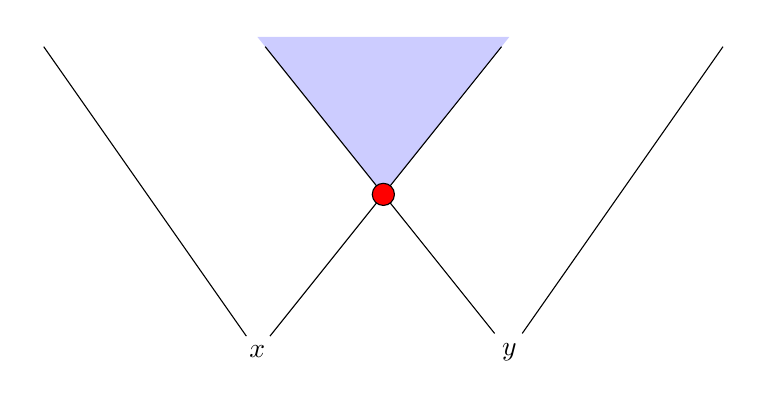
\begin{tikzpicture}[scale=0.8]
    % Nodes
    \node (from-y-to-x) at (-2, 5) {};
    \node (from-x-to-y) at (2, 5) {};
    \node (inters) at (0,2.5) {};
    \node (x-side) at (-5.5,5) {};
    \node (y-side) at (5.5,5) {};
    \node (x) at (-2,0) {$x$};
    \node (y) at (2,0) {$y$};

    %colorare l'area 
    \fill[blue!20] (0,2.5) -- (from-x-to-y.center) -- (from-y-to-x.center) -- cycle;
    

    % Lines
    \draw (x) -- (from-x-to-y);
    \draw (y) -- (from-y-to-x);
    \draw (x) -- (x-side);
    \draw (y) -- (y-side);

    \draw[fill=red] (0,2.5) circle (5pt);
    
  \end{tikzpicture}
\end{figure}
\subsubsection{Greatest lower bound}
Il greatest lower bound (\verb|GLB|) di un insieme di elementi è il più grande
elemento del reticolo che è minore o uguale a ciascun elemento dell'insieme ($X \land Y$).
Ovvero in $\wp(D)$ tale che $A \subseteq X$ e $A \subseteq Y$.
\begin{figure}[H]
  \centering
  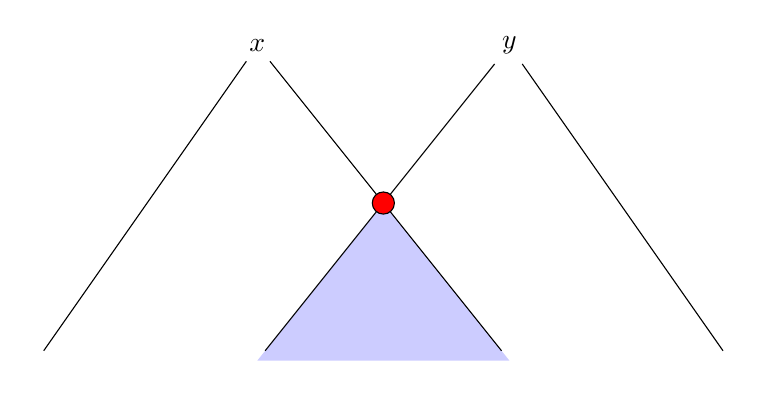
\begin{tikzpicture}[scale=0.8]
    % Nodes
    \node (from-y-to-x) at (-2, -5) {};
    \node (from-x-to-y) at (2, -5) {};
    \node (inters) at (0,-2.5) {};
    \node (x-side) at (-5.5,-5) {};
    \node (y-side) at (5.5,-5) {};
    \node (x) at (-2,0) {$x$};
    \node (y) at (2,0) {$y$};

    %colorare l'area 
    \fill[blue!20] (0,-2.5) -- (from-x-to-y.center) -- (from-y-to-x.center) -- cycle;
    

    % Lines
    \draw (x) -- (from-x-to-y);
    \draw (y) -- (from-y-to-x);
    \draw (x) -- (x-side);
    \draw (y) -- (y-side);

    \draw[fill=red] (0,-2.5) circle (5pt);
    
  \end{tikzpicture}
\end{figure}
\section{Approssimazione di $P$}
Sia $P^\#$ una proprietà di $D$ se e solo se $P^\#$ e $\wp(D)$. Vogliamo quindi capire la relazione tra gli 
elementi di $D$ e $\wp(D)$ e poi, preso $D^\# \subseteq \wp(D)$ la relazione tra gli elementi di $D$ e gli elementi 
di $D^\#$.
Per approssimare $D$ scegliamo un sottoinsieme $D^\#$ che fissa le proprietà che vogliamo osservare (\textit{con precisione}).
In generale $d \in D \implies d^\# \in D \subseteq \wp(D)$.

Potremmo quindi avere:
\begin{itemize}
  \item $d \subseteq d^\#$ ovvero \textbf{over approximation}.
  \item $d \supseteq d^\#$ ovvero \textbf{under approximation}.
\end{itemize}
\subsection{Approssimazione dal basso}
\begin{figure}[H]
  \centering
  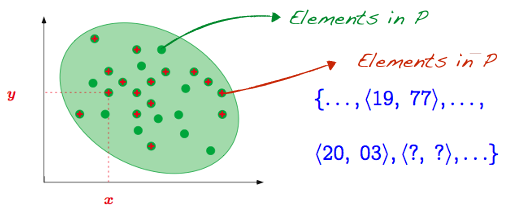
\includegraphics[scale=0.5]{img/approx.png}
\end{figure}
Per rispondere alla domanda $\langle x, y \rangle \in P$ utilizziamo un'astrazione $\bar{P}$,
tale che $P \supseteq \bar{P}$.
\begin{itemize}
  \item Se $\langle x, y \rangle \in \bar{P}$, quindi $d \subseteq d^\#$, allora $\langle x, y \rangle \in P$.
  \item Se $\langle x, y \rangle \notin \bar{P}$, quindi $d \supseteq d^\#$, allora non lo sappiamo.
\end{itemize}
In sintesi prendiamo un insieme più piccolo che comprende una sottoparte del nostro insieme di partenza e
analizziamo tale insieme più piccolo. Se troviamo una risposta positiva allora abbiamo risposto alla domanda,
altrimenti non lo sappiamo.
\subsection{Approssimazione dall'alto}
\begin{figure}[H]
  \centering
  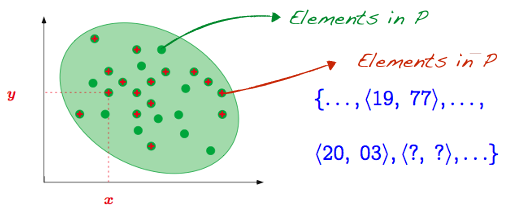
\includegraphics[scale=0.5]{img/approx.png}
\end{figure}
Per rispondere alla domanda $\langle x, y \rangle \in P$ utilizziamo un'astrazione $\bar{P}$,
tale che $P \subseteq \bar{P}$.
\begin{itemize}
  \item Se $\langle x, y \rangle \in \bar{P}$, quindi $d \supseteq d^\#$, allora non sappiamo rispondere.
  \item Se $\langle x, y \rangle \notin \bar{P}$, quindi $d \subseteq d^\#$, allora no.
\end{itemize}
In sintesi prendiamo un insieme più grande che comprende il nostro insieme di partenza e
analizziamo tale insieme più grande. Più grande non è sinonimo di più complesso, ma spesso 
ricondurci a proprietà più generali potrebbe aiutarci nell'analisi, la rappresentazione estensionale 
potrebbe quindi risultare più semplice. Tale approccio ci permette 
di rispondere alla domanda solo che la proprietà non è soddisfatta per il nuovo insieme più grande, 
ovvero $P^\#$.

In sostanza:
\begin{tcolorbox}[title=Proprietà concrete]
Le proprietà concrete sono un insieme di oggetti potenzialmente complessi, infiniti e non rappresentabili
da un calcolatore.
\end{tcolorbox}

\begin{tcolorbox}[title=Proprietà astratte]
  Le proprietà astratte sono un insieme più ampio di oggetti. A volte, l'ampiezza maggiore
  implica una maggiore estensibilità per la rappresentazione. Tuttavia, strutture più ampie
  ben scelte possono
  avere codifiche più semplici che possono essere sfruttate per la memorizzazione e il calcolo.
\end{tcolorbox}
\subsection{Minima astrazione}
Assumendo che le proprietà astratte $P \in \wp(\Sigma)$ devono essere apporssimate 
dall'alto della proprietà astratta $\bar{P} \in A \subset \wp(\Sigma)$, tale che:
\[
  P \subseteq \bar{P}
\]
Sappiamo che la più piccola proprietà $\bar{P}$ è la più precisa delle approssimazioni che possiamo avere.
Ovviamente, la minima proprietà astratta potrebbe non non esistere per tutte le astrazioni $A$.
Se questa minima approssimazione esiste è preferibile che sia il più precisa possibile, se non esiste,
può essere utilizzata una
migliore alternativa che fornisce un'approssimazione più precisa.
\subsection{Miglior astrazione}
Una buona scelta per l'astrazione è quella che fornisce la
miglior approssimazione per ogni proprietà concreta
\[
  P \subseteq \bar{P}
\]
\[
  \forall \bar{P}' \in A . (P \subseteq \bar{P}') \implies (\bar{P} \subseteq \bar{P}')
\]
Segue che la miglior approssimazione è la \textit{greatest lower bound} di tutte le approssimazioni
delle proprietà.
\[
\bar{P} = \bigcap \{\bar{P}' \in A \mid P \subseteq \bar{P}'\} \in A
\]
Tra tutti gli elementi più piccoli di quelli in $X$, è il più grande.
\[
  x = \texttt{glb}X \subseteq P \iff \forall l \in P . (\forall y \in X. l \leq y) \implies x \geq l
\]
\section{Astrazione delle computazioni}